\chapter[Conversor]{Conversor Tensão frequência}

\section{Introdução}

\say{Conversores tensão-frequência(VFC) são osciladores de primeira ordem cuja a entrada é uma tensão analógica $V_{in}$ e tem como saída um sinal em frequência $f_0$ linearmente proporcional à tensão de entrada, portanto:
\begin{equation}
 f_0 = kV_{in}
 \label{eq01}
\end{equation}
 Eles geralmente são denominados conversores quase digitais devido à sua saída analógica traduzida em frequência.

Os VFCs geralmente são confundidos com osciladores controlados por tensão (VCOs), mas observe que os VFCs têm especificações de desempenho diferentes e mais rigorosas: os requisitos típicos são precisão de fator de alta escala e estabilidade com temperatura e tensão de alimentação, ampla faixa dinâmica e baixo erro de linearidade.} \cite{livroprincipal}

Há muitas abordagens para um VFC, na literatura a maioria se baseia no mesmo princípio de operação, que é a integração alternada da tensão de entrada que gera pulsos quando a tensão de saída se iguala à uma tensão de referência.
Os VFCs têm duas configurações principais, o multivibrador e o equilíbrio de carga. Suas diferenças podem ser vistas na atuação do circuito de controle: no multivibrador o circuito de controle impõe as tensões limite, ajustando a oscilação de tensão no capacitor, enquanto no equilíbrio de carga, o circuito de controle fixa a duração da fase de carga ou descarga.

O multivibrador é, geralmente, um conversor Corrente-Frequência(IFC) precedido pro um conversor Tensão-Corrente(VIC). Seu princípio de funcionamento e aplicação são bem simples e precisa de pouca potência, mas são menos precisos que o equilíbrio de carga.
O equilíbrio de carga pode ser síncrono ou assíncrono, ele é mais preciso que o multivibrador. Entretanto precisa de mais potência e o seu sinal de saída são trens de pulsos, diferente do multivibrador que é uma onda quadrada.
A escolha para o projeto da \textit{TAG} foi da abordagem do VFC multivibrador pela pouca potência necessária.

O diagrama na Fig. \ref{fig04} descreve o funcionamento do VFC projetado. Nele, uma tensão de entrada $V_{in}$ é aplicada num conversor tensão corrente, essa corrente é espelhada no circuito integrador bidirecional que manda o sinal de tensão para um circuito de controle que, realimenta o integrador com os comandos de carga e descarga do capacitor no integrador.

\begin{figure}[htb]
	\centering
	\includegraphics[width=0.9\textwidth]{figuras/blocks_diagram_vf.png}
	\caption{Diagrama de blocos VFC Multivibrador Fonte:\cite{livroprincipal} }
	\label{fig04}
\end{figure}



\begin{figure}[htb]
	\centering
	\includegraphics[width=0.6\textwidth]{figuras/sch_diagrama.png}
	\caption{Esquemático VFC Multivibrador Fonte:\cite{livroprincipal} }
	\label{fig05}
\end{figure}

\begin{figure}[htb]
	\centering
	\includegraphics[width=0.6\textwidth]{figuras/formas_ondas.png}
	\caption{Formas de onda do Capacitor e Saída do VFC Multivibrador Fonte:\cite{livroprincipal} }
	\label{fig06}
\end{figure}

Na Fig. \ref{fig05} há um exemplo implementado do modelo de VFC multivibrador funcional. Nele uma fonte de corrente controlada pela tensão de entrada $V_{in}$ gera uma corrente que é integrada num capacitor aterrado cuja as tensões variam entre duas referências, a tensão menor $V_L$ e a maior $V_H$. Ao observar a tensão no capacitor o circuito de controle atua no sentido de carga e descarga e também envia o sinal digital de saída com a frequência correspondente à tensão de entrada.  
A frequência de saída é obtida na onda exibida na Fig. \ref{fig06} onde o sinal digital acompanha as retas de subida e descida na tensão do capacitor do integrador. A sua expressão é dada na Eq. \ref{eq01}. 

\section{Conversor Tensão corrente} 

O conversor tensão corrente(VIC) é um bloco base para muitos designs de sinais analógicos e mistos como em multiplicadores, conversores de dados, amplificadores de ganho variável.O VIC é o estágio de entrada do VFC, a maior parte  da performance depende desse bloco. Isso leva à necessidade de uma transcondutância($gm$) independente de temperatura, tempo e tensão com variação linear e largura de banda apropriada.\cite{livroprincipal}.

A ideia descrita nos artigos \cite{artigo_principal} e \cite{artigo_tag_unb} em que o trabalho se baseia é que para a análise dos sinais vitais a tensão gerada pelos batimentos cardíacos é retificada e então é usada como a tensão de entrada $V_{in}$ do VFC. 

\begin{figure}[htb]
%\begin{center}
	\centering
	\begin{circuitikz}[american,scale=0.8, transform shape]
%Há comandos que podem te auxiliar na exibição do seu circuito
\ctikzset{tripoles/mos style=arrows} % este coloca as pontas nos transistores
%\ctikzset{transistors/arrow pos=end}
%\ctikzflipxy{NAME} % Esse espelha o nome do componente que foi jirado nos eixos x e y
%\ctikzflipx{NAME} % Esse espelha os nome só no eixo x
%\ctikzflipy{NAME} % e esse só no eixo y
\draw (1.7,-6.3) node[nmos, rotate=180, yscale=-1 ] (N1) {\rotatebox{0}{\ctikzflipx{N1}}};
\draw (1.7,-8) node[nmos, rotate=180, yscale=-1 ] (N2) {\rotatebox{0}{\ctikzflipx{N2}}};
\draw (1.7,-9.7) node[nmos, rotate=180, yscale=-1 ] (N3) {\rotatebox{0}{\ctikzflipx{N3}}};
\draw (1.7,-11.3) node[nmos, rotate=180, yscale=-1 ] (N4) {\rotatebox{0}{\ctikzflipx{N4}}};
\draw (14.7,-3.3) node[pmos, rotate=0] (P5) {P5};
\draw (17.7,-3) node[pmos, rotate=180, yscale=-1 ] (P6) {\rotatebox{0}{\ctikzflipx{P6}}};

\draw (7.3,-8.7) node[nmos, rotate=180, yscale=-1 ] (N5) {\rotatebox{0}{\ctikzflipx{N5}}};
\draw (11.7,-8.7) node[nmos, rotate=0] (N6) {N6};
\draw (14.7,-7.7) node[nmos, rotate=180, yscale=-1 ] (N7) {\rotatebox{0}{\ctikzflipx{N7}}};
\draw (17.7,-7.7) node[nmos, rotate=0] (N8) {N8};
\draw (1.7,-2.3) node[pmos, rotate=180, yscale=-1 ] (P1) {\rotatebox{0}{\ctikzflipx{P1}}};
\draw (5,-4.7) node[pmos, rotate=0] (P2) {P2};
\draw (7.3,-2) node[pmos, rotate=180, yscale=-1 ] (P4) {\rotatebox{0}{\ctikzflipx{P4}}};
\draw (11.7,-2) node[pmos, rotate=0] (P3) {P3};

%VCCs
\draw (P1.S) -- (1.7,-1) node[vcc] {$V_{IN}$};
\draw (P2.S) -- (5,-1) node[vcc] {$V_{IN}$};
\draw (P3.S) -- (11.7,-1) node[vcc] {$V_{IN}$};
\draw (P4.S) -- (7.3,-1) node[vcc] {$V_{IN}$};
\draw (P5.S) -- (14.7,-1) node[vcc] {$V_{IN}$};

\draw (P6.S) -- (17.7,-1) node[vcc] {$V_{CC}$};


\draw  (P1.D) |-  (N1.D);
\draw  (N1.S) |-  (N2.D);
\draw  (N2.S) |-  (N3.D);
\draw  (N3.S) |-  (N4.D);
\draw  (N4.S) |- (1.7,-12) node[ground] {}; %(1.7,-16.2);
\draw  (N1.D) ++(0,1) coordinate(N1D);
\draw  (N1.G) |- (N1.D) node[circ] {};
\draw  (N2.G) |- (N2.D) node[circ] {};
\draw  (N3.G) |- (N3.D) node[circ] {};
\draw  (N4.G) |- (N4.D) node[circ] {};
\draw	 (N1D)  |- node[circ,midway] {} (P2.G);
%N5-6 
\draw  (N5.S) |- (7.3,-9.5) to[R=R] (7.3,-12) node[ground] {};
\draw  (N5.G)  -|  (N6.G);
\draw  (N6.S) |- (11.7,-12) node[ground] {};
\draw  (N6.G) ++(-0.7,0) node[circ] {}  -- ++(0,1) node[circ] {} coordinate(N26) -| node[circ,midway] {} (N6.D);
\draw  (P2.D) |- (N26);

\draw (P4.G) ++(0.6,0) node[circ] {} -- ++(0,-1.3) coordinate(P14) -| node[circ] {} (P4.D);
\draw (P1.G) -- ++(3,0) |- (P14);
\draw (P5.G) -| node[circ] {} (P14);

\draw (P6.G) |- (P6.D) node[circ] {};
\draw (P6.G) -- ++(1.5,0) node[vcc,rotate=-90,label=south west:$V_{OUT}$] {};

\draw  (N7.G) node[circ] {} |- (N7.D) node[circ] {};
\draw  (N7.S) |- (14.7,-12) node[ground] {};
\draw  (N7.G)  -|  (N8.G);
\draw  (N8.S) |- (17.7,-12) node[ground] {};

\draw  (P6.D) |-  (N8.D);
\draw  (P5.D) |-  (N7.D);
\draw  (P3.D) |-  (N6.D);
\draw  (P4.D) |-  (N5.D);
\draw  (P4.G)  -|  (P3.G);

\draw[thick,dashed] (6,-8) rectangle (9,-12);

	
	\end{circuitikz}
%	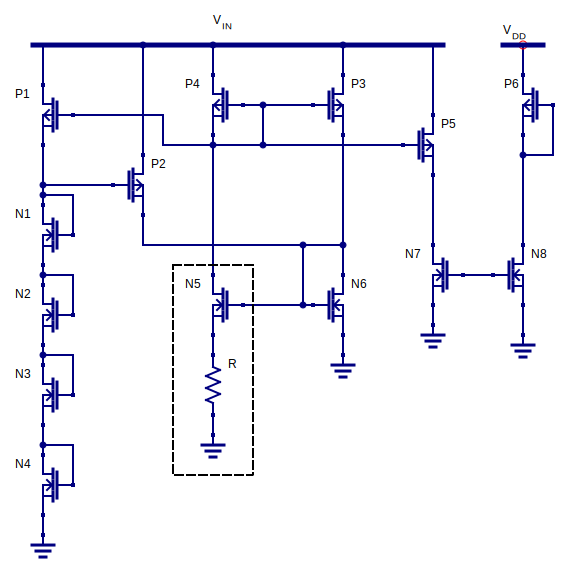
\includegraphics[width=0.8\textwidth]{figuras/v-i.png}
	\caption{Esquemático circuito conversor tensão corrente. Fonte:\cite{artigo_principal} }
	\label{fig07}
%\end{center}
\end{figure}

A topologia do circuito VIC desse projeto está exibida na Fig. \ref{fig07}. Observa-se no esquemático uma variação de uma bootstrapped auto-bias current source, ou seja, fonte de correte auto enviesada. Nesse modelo a corrente, limitada pelo resistor, é espelhada de forma mútua entre os espelhos dos PMOS $P_3$ e $P_4$  e NMOS $N_5$ e $N_6$. 
A relação à esquerda, composta pelo divisor de tensão com $P_1$, $P_2$, $N_1$ até $N_4$, funciona como um soft-start que regula a corrente de acordo com a variação da tensão $V_{in}$ de forma proporcional às tensões do $P_2$. Essas razões de proporção estão expressas na eq. \ref{eq02}.

\begin{equation}
 V_{in}\propto V_{GS,P2}\propto V_{GS,N6} = V_{GS,N5} \Rightarrow V_{in}\propto V_{GS,N5} \approx \frac{1}{R}
 \label{eq02}
\end{equation}


\begin{table}[htb]
\centering
\begin{tabular}{c|c}
\hline 
\hline 
\textbf{Nome do componente} & \textbf{Dimensões (W/L)[$\mu$ m]} \\ 
\hline 
\hline 
$P_1$, $N_1$,$N_2$,$N_3$,$N_4$ & 1/5 \\ 
\hline 
$P_2$ & 0.24/0.18 \\ 
\hline 
$P_3$, $P_4$, $P_5$  & 0.24/21.82 \\ 
\hline 
$N_5$,$N_6$ & 15/45 \\ 
\hline 
$N_7$,$N_8$ & 0.24/20 \\ 
\hline 
$P_6$ & 100/2 \\ 
\hline 
$R$ & 200 $\Omega$ \\ 
\hline 
\end{tabular} 
\caption{Dimensões dos transistores e resistor do VIC}
\label{tab:vic}
\end{table}

 Á direita da fonte há um espelho, composto por $N_7$ e $N_8$, que direciona uma corrente que será espelhada novamente para uma relação, $P_6$ e $N_8$, cuja a tensão de alimentação não é mais a $V_{in}$, que é traduzida em corrente, mas sim a tensão $V_{DD}$ padrão de alimentação do resto do circuito. Essa tensão de saída é a tensão de Bias usada nos espelhos para o circuito integrador usado para criar o sinal de frequência.

Considerações devem ser feitas sobre esse circuito. O primeiro é sobre a faixa de corrente que ele vai abranger, que exerce influência direta nas frequências de saída. Além disso quanto maior essa faixa maior será a potência consumida. A potência máxima exigida no projeto pode afetar o desenvolvimento do projeto para se ajustar ao consumo total essas faixas podem ser revistas.

 O controle dessa faixa é feito com o dimensionamento dos transistores e depois do resistor. Sua linearidade é controlada com a relação W/L que deve ser pequena para evitar efeitos de canal curto. Entretanto isso afeta no ganho e na transcondutância tornando a faixa menor. O controle da transcondutância também é influenciado pelo resistor, que de acordo com o seu tamanho ele aumenta ou reduz a faixa de corrente. Portanto deve-se procurar um equilíbrio comum entre essas parâmetros para que um não se sobressaia e afete demais o outro.


\section{Integrador} 

O integrador bidirecional é um circuito de carga/descarga com um capacitor $C$ temporizado e uma fonte de corrente constante que carrega o capacitor e um dissipador constante que o descarrega. O controle da carga e descarga do capacitor é feito com um circuito que observa a tensão no capacitor e a compara com tensões de referência limites, alto($V_H$) e baixo($V_L$), e dá a ordem de carga ou descarga. O acionamento é feito com a ativação alternada das chaves que selecionam a carga ou descarga. 
O modelo explicativo em blocos está na Fig. \ref{fig08}.

\begin{figure}[htb]
	\centering
	\includegraphics[width=0.5\textwidth]{figuras/integrador_sch.png}
	\caption{Integrador de corrente bidirecional com fonte e espelho de corrente. Fonte:\cite{livroprincipal} }
	\label{fig08}
\end{figure}

Na Fig. \ref{fig09} está o circuito proposto. Para destrinchar o seu funcionamento ignore momentaneamente os transistores $P_2$ e $P_3$. O transistor $P_1$ espelha a corrente do circuito VIC apresentado anteriormente e atua como uma fonte de corrente para o integrador. 
Inicialmente o capacitor está descarregado, com isso o sistema de controle faz o integrador ligar o $P_5$ e a corrente é direcionada no capacitor carregando-o. 
A tensão no capacitor então aumenta com a injeção de corrente nele seguindo a expressão da eq. \ref{eq03}. Sendo $V_0$ a tensão inicial ou anterior à mudança de estado do capacitor.

\begin{equation}
V_{cap}(t) = V_0 + \frac{I\cdot t}{C_1}
 \label{eq03}
\end{equation}

Após a tensão $V_{cap}$ atingir o valor de $V_H$ ele troca os estados das chaves deligando $P_5$ e acionando $P_4$. 
Assim a corrente agora é direcionada para o lado esquerdo que espelha a corrente nos transistores $N_2$ e $N_4$ descarregando o capacitor até atingir $V_L$ e o sistema de controle alternar as chaves de novo.  


A frequência do processo da carga e descarga é obtido com a expressão da eq. \ref{eq04}, que já é a expressão da frequência final observada no VFC, apesar da tensão do capacitor $V_{cap}$ não ser o sinal de saída do VFC. 

\begin{equation}
f = \frac{I}{C\cdot(V_H - V_L)}
 \label{eq04}
\end{equation}

\begin{figure}[htb]
	\centering
%Erro cometido nesse esquemático
%Os inversores de P4 e P5 não são ligados no GND, mas sim no Vbias
	%\includegraphics[width=0.7\textwidth]{figuras/integrate.png}
	\begin{circuitikz}[american,scale=0.7, transform shape] 
%Há comandos que podem te auxiliar na exibição do seu circuito
\ctikzset{tripoles/mos style=arrows} % este coloca as pontas nos transistores
%\ctikzset{transistors/arrow pos=end}
%\ctikzflipxy{NAME} % Esse espelha o nome do componente que foi jirado nos eixos x e y
%\ctikzflipx{NAME} % Esse espelha os nome só no eixo x
%\ctikzflipy{NAME} % e esse só no eixo y
\draw (16,-3.3) node[pmos, rotate=0] (P2) {P2};
\draw (13.3,-3.3) node[pmos, rotate=0] (P1) {P1};
\draw (18.7,-3.3) node[pmos, rotate=0] (P3) {P3};
\draw (13.3,-7.3) node[pmos, rotate=0] (P4) {P4};
\draw (11,-5.7) node[pmos, rotate=0] (P6) {P6};
\draw (11,-9) node[nmos, rotate=0] (N5) {N5};
\draw (18.7,-7.3) node[pmos, rotate=180, yscale=-1 ] (P5) {\rotatebox{0}{\ctikzflipx{P5}}};
\draw (21,-5.7) node[pmos, rotate=180, yscale=-1 ] (P7) {\rotatebox{0}{\ctikzflipx{P7}}};
\draw (21,-9) node[nmos, rotate=180, yscale=-1 ] (N6) {\rotatebox{0}{\ctikzflipx{N6}}};
\draw (13.3,-14.3) node[nmos, rotate=180, yscale=-1 ] (N1) {\rotatebox{0}{\ctikzflipx{N1}}};
\draw (18.7,-14.3) node[nmos, rotate=0] (N2) {N2};
\draw (13.3,-17) node[nmos, rotate=180, yscale=-1 ] (N3) {\rotatebox{0}{\ctikzflipx{N3}}};
\draw (18.7,-17) node[nmos, rotate=0] (N4) {N4};
\draw (18.7,-18) node[ground] {} -| (N4.S);
\draw (13.3,-18) node[ground] {} -| (N3.S);
\draw (21.7,-15) node[ground] {};
\draw (21.7,-13) to[C=C1] (21.7,-15);
\draw (10.7,-15) node[pmos, rotate=0] (P9) {P9};
\draw (10.7,-13) node[pmos, rotate=0] (P8) {P8};
\draw (10.7,-17) node[pmos, rotate=0] (P10) {P10};
\draw (10.7,-18) node[ground] {} node[circ] {};
%\draw  (16,-1.3) |-  (P2.S);%(16,-2.3);
\draw  (13.3,-5.7) to[short] (16,-5.7);
%\draw  (13.3,-1.3) |-  (P1.S);%(13.3,-2.3);

\draw  (9.3,-3.3) node[ocirc,label=$V_{in}$] {} -| (P1.G);%(12.3,-3.3);
\draw[arrows = {-Stealth[scale width=1.5]}] (9.3,-3.3) node[ocirc] {} -- ++(0.8,0);

\draw  (P2.G)  -|  (P3.G);
%\draw  (18.7,-1.3) |-  (P3.S);%(18.7,-2.3);
\draw  (P1.G)  -|  (P2.G);
\draw  (P1.D) |- (13.3,-5.7);
\draw  (16,-5.7) to[short] (18.7,-5.7);
\draw  (P2.D) |- (16,-5.7);
\draw (16,-5.7)node[circ] {} coordinate(O0);
\draw  (P3.D) |- (18.7,-5.7);
\draw  (13.3,-5.7) |-  (P4.S);%(13.3,-6.3);
\draw (13.3,-5.7)node[circ] {} coordinate(O1);
\draw  (11,-7.3) -|  (P4.G);%(12.3,-7.3);
\draw  (P6.D) |- (11,-7.3);
\draw  (11,-7.3) |-  (N5.D);%(11,-8);
\draw (11,-7.3)node[circ] {} coordinate(O2);
\draw  (P6.G)  |-  (N5.G);
\draw  (18.7,-5.7) |-  (P5.S);%(18.7,-6.3);
\draw (18.7,-5.7)node[circ] {} coordinate(O3);
\draw  (P5.G)  -| (21,-7.3);
\draw  (P7.D) |- (21,-7.3);
\draw  (21,-7.3) |-  (N6.D);%(21,-8);
\draw (21,-7.3)node[circ] {} coordinate(O4);
\draw  (P7.G)  |-  (N6.G);
\draw  (N1.G)  -|  (N2.G);
\draw  (P4.D) |- (13.3,-12.7);
\draw  (13.3,-12.7) |-  (N1.D);%(13.3,-13.3);
\draw  (13.3,-12.7) to[short] (15.3,-12.7);
\draw (13.3,-12.7)node[circ] {} coordinate(O5);
\draw  (15.3,-12.7) to[short] (15.3,-17);
\draw  (N2.S) |-  (N4.D);
\draw  (N1.S) |-  (N3.D);
\draw  (N3.G)  -| (15.3,-17);
\draw  (15.3,-17) -|  (N4.G);%(17.7,-17);
\draw (15.3,-17)node[circ] {} coordinate(O6);
\draw  (P5.D) |- (18.7,-12.3);
\draw  (18.7,-12.3) |-  (N2.D);%(18.7,-13.3);
\draw  (18.7,-12.3) to[short] (21.7,-12.3);
\draw (18.7,-12.3)node[circ] {} coordinate(O7);

\draw (21.7,-12.3) -- ++(0.5,0) node[ocirc,label=right:$V_{CAP}$] {};

\draw  (21.7,-12.3) to[short] (21.7,-13);
\draw  (9.7,-14)  -| node[circ,midway] {} (P9.S);%(10.7,-14);
\draw  (P8.G)  |- (9.7,-14) coordinate(P89);
\draw  (P9.G)  |- (9.7,-16) coordinate(P910);
\draw  (9.7,-16) -|  (P9.D);%(10.7,-16);
\draw  (P10.G)  |-  (9.7,-18);
\draw  (9.7,-18) -|  (P10.D);%(10.7,-18);
\draw  (N5.S) |-  (N5.S);
\draw  (P6.S) |-  (P6.S);
\draw  (P7.S) |-  (P7.S);
\draw  (N6.S) |-  (N6.S);
\draw  (P8.S) |-  (P8.S);
\draw  (16,-1.3) to[short] (16,-1.3);
\draw  (13.3,-1.3) to[short] (13.3,-1.3);
\draw  (9.3,-3.3) to[short] (9.3,-3.3);
\draw  (18.7,-1.3) to[short] (18.7,-1.3);
\draw  (P9.S)  -|  (P8.D);
\draw  (P910)  -| node[circ,midway] {} (P10.S);
\draw  (P9.G)  -- ++(-0.5,0) node[ocirc,label=$V_{bias}$] {};
\draw  (N2.G) -- ++(-1.7,0) -- ++(0,0.5) node[ocirc,label=$V_{bias}$] {};
\draw  (N5.S) -- ++(0,-0.5)  node[ocirc,label=left:$V_{bias}$] {};
\draw  (N6.S) -- ++(0,-0.5)  node[ocirc,label=left:$V_{bias}$] {};

\draw[arrows = {Stealth[scale width=1.5]}-] (P6.G |- O2) node[circ] {} ++(-0.3,0) -- ++(-0.5,0) node[ocirc,label=below:NQ] {} -- (P6.G |- O2) ;

\draw[arrows = {Stealth[scale width=1.5]}-] (P7.G |- O4) node[circ] {} ++(0.3,0) -- ++(0.5,0) node[ocirc,label=below:Q] {} -- (P7.G |- O4);

\draw (P1.S) -- ++(0,0.5) node[vcc] {ADJ1};
\draw (P2.S) -- ++(0,0.5) node[vcc] {ADJ2};
\draw (P3.S) -- ++(0,0.5) node[vcc] {ADJ3};

\draw (P8.S) -- ++(0,0.5) node[vcc] {VDD};
\draw (P6.S) -- ++(0,0.5) node[vcc] {VDD};
\draw (P7.S) -- ++(0,0.5) node[vcc] {VDD};


\end{circuitikz}
	
	\caption{Esquemático do Integrador de Corrente Bidirecional Fonte:\cite{artigo_tag_unb} }
	\label{fig09}
\end{figure}

Os transistores $N_1$ e $N_2$ estão ativados com uma tensão de bias o suficiente para ligá-los. Os $P_2$ e $P_3$ são acionados para atingir novas faixas de frequência. A ideia é de que ao acionar cada um dos transistores que espelha a corrente do VIC a faixa mude entre as opções: 100Hz-1kHz, 1kHz-10kHz e 10kHz-100kHz. Onde as correntes de $P_2$ e $P_3$  são somadas para alterar as frequências no integrador.

\begin{table}[htb]
\centering
\begin{tabular}{c|c}
\hline 
\hline 
\textbf{Nome do componente} & \textbf{Dimensões (W/L)[$\mu$ m]} \\ 
\hline 
\hline 
$P_6$, $P_7$, $N_5$ ,$N_6$ & 0.24/0.18 \\ 
\hline 
$P_4$, $P_5$, $N_1$,$N_2$,$N_3$,$N_4$ & 1/15 \\ 
\hline 
$P_8$, $P_9$, $P_10$  & 0.3/0.18 \\ 
\hline 
$P_1$ & 0.73/2 \\ 
\hline 
$P_2$ & 6.5/2 \\ 
\hline 
$P_3$ & 73/2 \\ 
\hline 
$C$ & 7pF \\ 
\hline 
\end{tabular} 
\caption{Dimensões dos transistores e capacitor do Integrador bidirecional}
\label{tab:integrador}
\end{table}


\section{Circuito de Controle} 

O circuito de controle usado é baseado na topologia da Fig. \ref{fig10}, onde são usado dois AmpOps como comparadores da tensão $V_{cap}$ com os limiares $V_H$ e $V_L$ e os seus sinais são usados na entrada de um latch SR. O latch recebe a saída da relação de AmpOps e, com os sinais $Q$ e $NQ$ realimenta esses sinais no circuito integrador. A saída final do VFC é o sinal $Q$ do circuito de controle.


\begin{figure}[htb]
     \centering
     \begin{subfigure}[b]{0.49\textwidth}
         \centering
         \includegraphics[width=\textwidth]{figuras/control_topology.png}
         \caption{Topologia do circuito de controle.}
         \label{fig10}
     \end{subfigure}
     \hfill
     \begin{subfigure}[b]{0.49\textwidth}
         \centering
         \includegraphics[width=\textwidth]{figuras/controle_waves.jpg}
         \caption{Formas de onda dos sinais esperados no sistema de controle}
         \label{fig11}
     \end{subfigure}
        \caption{Fonte:\cite{livroprincipal}}
        \label{fig:control}
\end{figure}

Em simulação o bloco do circuito foi feito como apresentado na Fig. \ref{fig12}, onde as tensões $V_H$ e $V_L$ são obtidas com os divisores de tensão dos transistores conectados em diodo. No circuito dessa figura já está implementado ambos os AmpOps e o espelho de corrente usado para polarizá-los.

%\begin{figure}[htb]
%	\centering
%	%\includegraphics[width=0.9\textwidth]{figuras/controle.png}
%\begin{circuitikz}[american,scale=1, transform shape] 
%%Há comandos que podem te auxiliar na exibição do seu circuito
%\ctikzset{tripoles/mos style=arrows} % este coloca as pontas nos transistores
%%\ctikzset{transistors/arrow pos=end}
%%\ctikzflipxy{NAME} % Esse espelha o nome do componente que foi jirado nos eixos x e y
%%\ctikzflipx{NAME} % Esse espelha os nome só no eixo x
%%\ctikzflipy{NAME} % e esse só no eixo y

%\draw (7,6) node[pmos] (P1) {P1};
%\draw (7,4) node[pmos] (P2) {P2};
%\draw (7,2) node[pmos] (P3) {P3};

%\draw (10,6) node[pmos] (P4) {P4};
%\draw (10,4) node[pmos] (P5) {P5};
%\draw (10,2) node[pmos] (P6) {P6};

%\draw (P1.S) node[vcc] {VDD};
%\draw (P4.S) node[vcc] {VDD};

%\draw (P1.G) |- (P1.D);
%\draw (P2.G) |- (P2.D);
%\draw (P3.G) |- (P3.D);
%\draw (P1.D) -| (P2.S);
%\draw (P2.D) -| (P3.S);

%\draw (P4.G) |- (P4.D);
%\draw (P5.G) |- (P5.D);
%\draw (P6.G) |- (P6.D);
%\draw (P4.D) -| (P5.S);
%\draw (P5.D) -| (P6.S);

%\draw (P2.G) -- ++(-0.5,0) node[ocirc,label=left:$V_L$] {};
%\draw (P4.G) -- ++(-0.5,0) node[ocirc,label=left:$V_H$] {};

%\draw (P3.D) node[ground] {};
%\draw (P6.D) node[ground] {};

%\draw (0,6) node[op amp, noinv input up] (AH) {AH};
%\draw (0,2) node[op amp, noinv input up] (AL) {AL};
%\draw (3,4) node[flipflop SR] (SR) {Latch SR};

%\draw (AH.+) -- ++(-1,0) node[ocirc,label=left:$V_H$] {} coordinate(AHN);
%\draw (AL.-) -- ++(-1,0) node[ocirc,label=left:$V_L$] {} coordinate(ALI);

%\draw (AH.-) -- ++(-0.5,0) coordinate(aux) |- (AL.+);
%\draw (AHN |- SR) node[ocirc, label=left:$V_{CAP}$] {} -- (aux |- SR);

%\draw (AH.out) |- (SR.pin 1);
%\draw (AL.out) |- (SR.pin 3);

%\draw (AH.up) -- ++(0,0.5) node[vcc] {VDD};
%\draw (AL.up) -- ++(0,0.5) node[vcc] {VDD};

%\draw (AH.down) -- ++(0,-0.5) node[ground] {};
%\draw (AL.down) -- ++(0,-0.5) node[ground] {};


%\end{circuitikz}
%	\caption{Esquemático dos componentes do Circuito de controle acompanhados dos divisores de tensão para as tensões de Bias $V_H$ e $V_L$ Fonte:\cite{artigo_principal} }
%	\label{fig12}
%\end{figure}

\begin{figure}[H] 
\centering
\begin{circuitikz}[american,scale=0.6, transform shape] 
%Há comandos que podem te auxiliar na exibição do seu circuito
%\ctikzset{tripoles/mos style=arrows} % este coloca as pontas nos transistores
%\ctikzset{transistors/arrow pos=end}
%\ctikzflipxy{NAME} % Esse espelha o nome do componente que foi jirado nos eixos x e y
%\ctikzflipx{NAME} % Esse espelha os nome só no eixo x
%\ctikzflipy{NAME} % e esse só no eixo y
\draw (19,-2.3) node[pmos, rotate=0] (P1) {P1};
\draw (16.3,-6.3) node[pmos, rotate=0] (P2) {P2};
\draw (21.7,-6.3) node[pmos, rotate=180, yscale=-1 ] (P3) {\rotatebox{0}{\ctikzflipx{P3}}};
\draw (25.3,-2.3) node[pmos, rotate=0] (P4) {P4};
\draw (10.3,-2.3) node[pmos, rotate=180, yscale=-1 ] (P5) {\rotatebox{0}{\ctikzflipx{P5}}};
\draw (7.7,-6.3) node[pmos, rotate=0] (P6) {P6};
\draw (21.7,-10) node[nmos, rotate=0] (N2) {N2};
\draw (25.3,-8) node[nmos, rotate=0] (N3) {N3};
\draw (13,-6.3) node[pmos, rotate=180, yscale=-1 ] (P7) {\rotatebox{0}{\ctikzflipx{P7}}};
\draw (4,-2.3) node[pmos, rotate=180, yscale=-1 ] (P8) {\rotatebox{0}{\ctikzflipx{P8}}};
\draw (7.7,-10) node[nmos, rotate=180, yscale=-1 ] (N4) {\rotatebox{0}{\ctikzflipx{N4}}};
\draw (13,-10) node[nmos, rotate=0] (N5) {N5};
\draw (4,-8) node[nmos, rotate=180, yscale=-1 ] (N6) {\rotatebox{0}{\ctikzflipx{N6}}};
\draw (16.3,-19.3) node[pmos, rotate=0] (P12) {P12};
\draw (21.7,-19.3) node[pmos, rotate=0] (P15) {P15};
\draw (5.3,-19.3) node[nmos, rotate=180, yscale=-1 ] (N7) {\rotatebox{0}{\ctikzflipx{N7}}};
\draw (9.3,-19.3) node[nmos, rotate=0] (N8) {N8};
\draw (16.3,-20.7) node[ground] {};
\draw (21.7,-20.7) node[ground] {};
\draw (9.3,-20.7) node[ground] {};
\draw (5.3,-20.7) node[ground] {};
\draw (9.3,-14.7) node[pmos, rotate=180, yscale=-1 ] (P9) {\rotatebox{0}{\ctikzflipx{P9}}};
\draw (5.3,-13.7) node[vcc] {VDD} to[isource=I1] (5.3,-15.7);
\draw (21.7,-17) node[pmos, rotate=0] (P14) {P14};
\draw (21.7,-14.3) node[pmos, rotate=0] (P13) {P13};
\draw (16.3,-14.3) node[pmos, rotate=0] (P10) {P10};
\draw (16.3,-17) node[pmos, rotate=0] (P11) {P11};
\draw (7.7,-11.3) node[ground] {};
\draw (13,-11.3) node[ground] {};
\draw (4,-11.3) node[ground] {};
\draw (21.7,-11.3) node[ground] {};
\draw (16.3,-11.3) node[ground] {};
\draw (25.3,-11.3) node[ground] {};
\draw (16.3,-10) node[nmos, rotate=180, yscale=-1 ] (N1) {\rotatebox{0}{\ctikzflipx{N1}}};
\draw  (7.7,-4.7) to[short] (10.3,-4.7);
\draw  (10.3,-4.7) to[short] (13,-4.7);
\draw  (P5.D) |- (10.3,-4.7);
\draw (10.3,-4.7)node[circ] {} coordinate(O0);
\draw  (13,-4.7) |-  (P7.S);%(13,-5.3);
\draw  (7.7,-4.7) |-  (P6.S);%(7.7,-5.3);
\draw  (6,-6.3) node[currarrow, scale=2, xscale=1] {} node[left] {VL} -|  (P6.G);%(6.7,-6.3);
\draw  (P6.D) |- (7.7,-8.7);
\draw  (P8.G)  -|  (P5.G);
\draw  (P8.D) |- (4,-5.3);
\draw  (N4.G)  -| (9,-10);
\draw  (P7.D) |- (13,-8);
\draw  (16.3,-4.7) to[short] (19,-4.7);
\draw  (19,-4.7) to[short] (21.7,-4.7);
\draw  (P1.D) |- (19,-4.7);
\draw (19,-4.7)node[circ] {} coordinate(O1);
\draw  (16.3,-4.7) |-  (P2.S);%(16.3,-5.3);
\draw  (21.7,-4.7) |-  (P3.S);%(21.7,-5.3);
\draw  (P3.G)  -| (23.3,-6.3) node[currarrow, scale=2, xscale=-1] {} node[right] {VH};
\draw  (P3.D) |- (21.7,-8);
\draw  (P1.G)  -|  (P4.G);
\draw  (P4.D) |- (25.3,-5.3);
\draw  (21.7,-8) -|  (N3.G);%(24.3,-8);
\draw  (21.7,-8) |-  (N2.D);%(21.7,-9);
\draw (21.7,-8)node[circ] {} coordinate(O2);
\draw  (P2.D) |- (16.3,-8.7);
\draw  (N1.G)  -| (17.7,-10);
\draw  (P7.G)  -| (14.7,-6.3);
\draw  (14.7,-6.3) -|  (P2.G);%(15.3,-6.3);
\draw  (14.7,-4.7) node[trarrow,rotate=-90,xscale=1,scale=2] {} node[above] {$V_{cap}$} to[short] (14.7,-6.3);
\draw (14.7,-6.3)node[circ] {} coordinate(O3);
\draw  (P5.G)  -| (14.7,-2.3);
\draw  (P12.G)  |- (15.3,-20.3) ;
\draw  (15.3,-20.3) -| node[circ,midway] {} (P12.D);%(16.3,-20.3);
\draw  (P15.G)  |- (20.7,-20.3);
\draw  (20.7,-20.3) -| node[circ,midway] {} (P15.D);%(21.7,-20.3);
\draw  (N7.G)  -| (6.7,-19.3);
\draw  (6.7,-19.3) -|  (N8.G);%(8.3,-19.3);
\draw  (6.7,-18) to[short] (6.7,-19.3);
\draw (6.7,-19.3)node[circ] {} coordinate(O4);
\draw  (5.3,-18) |-  (N7.D);%(5.3,-18.3);
\draw  (5.3,-18) to[short] (6.7,-18);
\draw  (13,-8) |-  (N5.D);%(13,-9);
\draw  (N6.G)  -| (13,-8);
\draw (13,-8)node[circ] {} coordinate(O5);
\draw  (25.3,-5.3) |-  (N3.D);%(25.3,-7);
\draw  (25.3,-5.3)  to[short] (26.3,-5.3) node[currarrow, scale=2, xscale=1] {} node[right] {RES};
\draw (25.3,-5.3)node[circ] {} coordinate(O6);
\draw  (4,-5.3) |-  (N6.D);%(4,-7);
\draw  (3,-5.3) node[currarrow, scale=2, xscale=-1] {} node[left] {SET} to[short] (4,-5.3);
\draw (4,-5.3)node[circ] {} coordinate(O7);
\draw  (P12.D) |- (16.3,-20.7);
\draw  (P15.D) |- (21.7,-20.7);
\draw  (N8.S) |- (9.3,-20.7);
\draw  (N7.S) |- (5.3,-20.7);
\draw  (P9.D) |- (9.3,-16);
\draw  (P9.G)  -| (10.7,-14.7);
\draw  (10.7,-14.7) to[short] (10.7,-16);
\draw  (9.3,-16) |-  (N8.D);%(9.3,-18.3);
\draw  (9.3,-16) to[short] (10.7,-16);
\draw (9.3,-16)node[circ] {} coordinate(O8);
\draw  (5.3,-15.7) to[short] (5.3,-18);
\draw (5.3,-18)node[circ] {} coordinate(O9);
\draw  (P14.D) |-  (P15.S);
\draw  (20.3,-14.3) to[short] (20.3,-15.7);
\draw  (20.3,-14.3) -|  (P13.G);%(20.7,-14.3);
\draw  (21.7,-15.7) |-  (P14.S);%(21.7,-16);
\draw  (20.3,-15.7) to[short] (21.7,-15.7);
\draw  (19.7,-15.7) node[currarrow, scale=2, xscale=-1] {} node[left] {VH} to[short] (20.3,-15.7);
\draw (20.3,-15.7)node[circ] {} coordinate(O10);
\draw  (P13.D) |- (21.7,-15.7);
\draw (21.7,-15.7)node[circ] {} coordinate(O11);
\draw  (20.3,-17) -|  (P14.G);%(20.7,-17);
\draw  (20.3,-17) to[short] (20.3,-18.3);
\draw  (20.3,-18.3) -| node[circ,midway] {} (P15.S);%(21.7,-18.3);
\draw  (P10.D) |-  (P11.S);
\draw  (P11.D) |-  (P12.S);
\draw  (15,-18.3)  -|  node[circ,midway] {} (P12.S);%(16.3,-18.3);
\draw  (14.3,-17) node[currarrow, scale=2, xscale=-1] {} node[left] {VL} to[short] (15,-17);
\draw  (15,-17) -|  (P11.G);%(15.3,-17);
\draw  (15,-17) to[short] (15,-18.3);
\draw (15,-17)node[circ] {} coordinate(O12);
\draw  (P10.G)  |- (15.3,-15.3);
\draw  (15.3,-15.3) -| node[circ,midway] {} (P10.D);%(16.3,-15.3);
\draw  (N3.S) |- (25.3,-11.3);
\draw  (N2.S) |- (21.7,-11.3);
\draw  (N6.S) |- (4,-11.3);
\draw  (N5.S) |- (13,-11.3);
\draw  (N4.S) |- (7.7,-11.3);
\draw  (7.7,-8.7) |-  (N4.D);%(7.7,-9);
\draw  (7.7,-8.7) to[short] (9,-8.7);
\draw (7.7,-8.7)node[circ] {} coordinate(O13);
\draw  (9,-10) -|  (N5.G);%(12,-10);
\draw  (9,-8.7) to[short] (9,-10);
\draw (9,-10)node[circ] {} coordinate(O14);
\draw  (N1.S) |- (16.3,-11.3);
\draw  (16.3,-8.7) |-  (N1.D);%(16.3,-9);
\draw  (16.3,-8.7) to[short] (17.7,-8.7);
\draw (16.3,-8.7)node[circ] {} coordinate(O15);
\draw  (17.7,-10) -|  (N2.G);%(20.7,-10);
\draw  (17.7,-8.7) to[short] (17.7,-10);
\draw (17.7,-10)node[circ] {} coordinate(O16);
\draw  (10.7,-14.7) to[short] (11,-14.7) node[trarrow,xscale=1,scale=2] {} node[right] {$V_{biasP}$};
\draw (10.7,-14.7)node[circ] {} coordinate(O17);
\draw  (14.7,-2.3) -|  (P1.G);%(18,-2.3);
\draw  (14.7,-2) ++(0,0.6) node[inputarrow,rotate=-90,xscale=1,scale=2] {}  node[left] {$V_{biasP}$} to[short] (14.7,-2.3);
\draw (14.7,-2.3)node[circ] {} coordinate(O18);
\draw  (P1.S) node[vcc]{VDD};
\draw  (P4.S) node[vcc]{VDD};
\draw  (P5.S) node[vcc]{VDD};
\draw  (P8.S) node[vcc]{VDD};
\draw  (P9.S) node[vcc]{VDD};
\draw  (5.3,-13.7) to[short] (5.3,-13.7);
\draw  (P13.S) node[vcc]{VDD};
\draw  (P10.S) node[vcc]{VDD};
\draw  (6,-6.3) to[short] (6,-6.3);
\draw  (23.3,-6.3) to[short] (23.3,-6.3);
\draw  (14.7,-4.7) to[short] (14.7,-4.7);
\draw  (26.3,-5.3) to[short] (26.3,-5.3);
\draw  (3,-5.3) to[short] (3,-5.3);
\draw  (19.7,-15.7) to[short] (19.7,-15.7);
\draw  (14.3,-17) to[short] (14.3,-17);
\draw  (11,-14.7) to[short] (11,-14.7);
\draw  (14.7,-2) to[short] (14.7,-2);
\end{circuitikz} 
	\caption{Esquemático do circuito de controle feito com transistores e acompanhados do espelho de corrente e dos divisores de tensão para as tensões de Bias $V_H$ e $V_L$ Fonte:\cite{artigo_principal}}
	\label{fig12}
\end{figure}

\begin{table}[htb]
\centering
\begin{tabular}{c|c}
\hline 
\hline 
\textbf{Nome do componente} & \textbf{Dimensões (W/L)[$\mu$ m]} \\ 
\hline 
\hline 
$P_{1}$, $P_{4}$, $P_{5}$, $P_{8}$, $P_{9}$ & 0.4/0.2 \\ \hline
$P_{2}$, $P_{3}$, $P_{6}$, $P_{7}$, $N_{1}$, $N_{2}$, $N_{3}$, $N_{4}$, $N_{5}$, $N_{6}$  & 0.24/0.18 \\ \hline
$N_7$ & 10/1 \\ \hline
$N_{8}$ & 1/1 \\ \hline

$P_13$ & 1/2 \\ \hline 
$P_{10}$, $P_{11}$, $P_{12}$, $P_{14}$, $P_{15}$  & 1/5 \\ 
\hline 
\end{tabular} 
\caption{Dimensões dos transistores para o circuito de controle da Fig\ref{fig12}}
\label{tab:control}
\end{table}

\subsection{Latch SR}

O Latch SR pode ser descrito como um circuito digital primitivo de memória. Com ele é possível manusear estados e por tabela armazenar informação. Há dois tipos de Latch SR, o que se baseia em portas lógicas NOR e NAND.
O comportamento lógico desse circuito está descrito nas tabelas verdade das figuras \ref{fig13} e \ref{fig14}. Em resumo o do tipo NAND foi usado no projeto por conta do seu estado ser alterado para as condições desejadas no controlador com a queda nos sinais de SET($S$) e RESET($R$). Há abordagens que usa o Latch de tipo NOR, mas com inversores na entrada, isso é observado na Fig. \ref{fig10} por exemplo. 
O circuito do Latch SR montado a partir dos transistores MOS se encontra na Fig. \ref{fig15}. 


\begin{figure}[htb]
     \centering
     \begin{subfigure}[b]{0.49\textwidth}
         \centering
         \includegraphics[width=\textwidth]{figuras/lacthSR_NOR.png}
         \caption{Esquemático Latch SR tipo NOR}
         \label{fig13}
     \end{subfigure}
     \hfill
     \begin{subfigure}[b]{0.49\textwidth}
         \centering
         \includegraphics[width=\textwidth]{figuras/lachSR_NAND.png}
         \caption{Esquemático Latch SR tipo NAND}
         \label{fig14}
     \end{subfigure}
        \caption{Fonte:\cite{cmos_digital}}
        \label{fig:latch}
\end{figure}


\begin{figure}[htb]
	\centering
	%\includegraphics[width=0.9\textwidth]{figuras/lach_sr_NAND.png}
\begin{circuitikz}[american,scale=0.8, transform shape] 
%Há comandos que podem te auxiliar na exibição do seu circuito
\ctikzset{tripoles/mos style=arrows} % este coloca as pontas nos transistores
%\ctikzset{transistors/arrow pos=end}
%\ctikzflipxy{NAME} % Esse espelha o nome do componente que foi jirado nos eixos x e y
%\ctikzflipx{NAME} % Esse espelha os nome só no eixo x
%\ctikzflipy{NAME} % e esse só no eixo y
\draw (17,-6) node[pmos, rotate=180, yscale=-1 ] (P2) {\rotatebox{0}{\ctikzflipx{P2}}};
\draw (13.3,-6) node[pmos, rotate=0] (P1) {P1};
\draw (15.3,-9.3) node[nmos, rotate=0] (N1) {N1};
\draw (15.3,-12) node[nmos, rotate=180, yscale=-1 ] (N2) {\rotatebox{0}{\ctikzflipx{N2}}};
\draw (24,-6) node[pmos, rotate=180, yscale=-1 ] (P3) {\rotatebox{0}{\ctikzflipx{P3}}};
\draw (20.3,-6) node[pmos, rotate=0] (P4) {P4};
\draw (22.3,-9.3) node[nmos, rotate=0] (N3) {N3};

\draw (22.3,-12) node[nmos, rotate=180, yscale=-1 ] (N4) {\rotatebox{0}{\ctikzflipx{N4}}};
\draw  (P1.D) |- (15.3,-7);
\draw  (15.3,-7) -|  (P2.D);%(17,-7);
\draw  (15.3,-7) to[short] (15.3,-7.3);
\draw (15.3,-7)node[circ] {} coordinate(O0);
\draw  (N1.S) |-  (N2.D);
\draw  (P1.S) -|  (P2.S);
\draw  (12,-9.3) -|  (N1.G);%(14.3,-9.3);
\draw  (12,-6) to[short] (12,-9.3);
\draw  (12,-6) -|  (P1.G);%(12.3,-6);
\draw  (N2.G)  -| (18.3,-12);
\draw  (P2.G)  -| (18.3,-6);
\draw  (18.3,-6) to[short] (18.3,-8.3);
\draw  (15.3,-7.3) |-  (N1.D);%(15.3,-8.3);
\draw  (18.3,-8.3) to[short] (18.3,-12);
\draw  (15.3,-7.3) to[short] (19,-7.3);
\draw (15.3,-7.3)node[circ] {} coordinate(O1);

\draw  (18.3,-8.3) -- ++(2,0) -- ++(0,0.5) node[ocirc,label=north:$NQ$] {} -- ++(0,-0.5) -| node[circ] {}  (N3.D);%(22.3,-8.3);

\draw (18.3,-8.3)node[circ] {} coordinate(O2);
\draw  (P4.D) |- (22.3,-7);
\draw  (22.3,-7) -|  (P3.D);%(24,-7);
\draw  (22.3,-7) |-  (N3.D);%(22.3,-8.3);
\draw (22.3,-7)node[circ] {} coordinate(O3);
\draw  (N3.S) |-  (N4.D);
\draw  (P4.S) -|  (P3.S);
\draw  (19,-9.3) -|  (N3.G);%(21.3,-9.3);
\draw  (19,-6) to[short] (19,-7.3);
\draw  (19,-6) -|  (P4.G);%(19.3,-6);
\draw  (N4.G)  -| (25.3,-12);
\draw  (P3.G)  -| (25.3,-6);
\draw  (25.3,-6) to[short] (25.3,-12);
\draw  (19,-7.3) to[short] (19,-9.3);
\draw (19,-7.3)node[circ] {} coordinate(O4);

\draw  (O4) -- ++(-2,0) -- ++(0,-0.5) node[ocirc,label=below:$Q$] {} ;
\draw  (12,-9.3) -- ++(0,-0.5) node[ocirc, label=right:$SET$] {};
\draw (N2.S) -- (15.3,-13) node[ground] {};
\draw (N4.S) -- (22.3,-13) node[ground] {};
\draw (25.3,-12) -- ++ (0.5,0) node[ocirc,label=right:$RES$] {};

\end{circuitikz}
	\caption{Topologia Latch SR do tipo NAND Fonte:\cite{cmos_digital} }
	\label{fig15}
\end{figure}

\begin{table}[htb]
\centering
\begin{tabular}{c|c}
\hline 
\hline 
\textbf{Nome do componente} & \textbf{Dimensões (W/L)[$\mu$ m]} \\ 
\hline 
\hline 
$P_1$, $P_2$, $P_3$, $P_4$ 	& 2.65/0.18 \\ \hline 
$N_1$, $N_2$, $N_3$, $N_4$  & 0.24/0.18 \\ 
\hline 
\end{tabular} 
\caption{Dimensões dos transistores do Latch SR NAND}
\label{tab:latch}
\end{table}

\newpage

\subsection{Amplificador operacional}

Os comparadores do circuito de controle são AmpOps. Para cada AmpOp foi usado a topologia de 2 estágios com conexão diodo, como observado na Fig.\ref{fig16}. A tensão de Bias, $V_{biasP}$, para polarização dos transistores $P_1$ e $P_4$ é feita com o espelho de corrente usando a fonte de tensão do projeto Cedro.

O ganho dessa topologia de AmpOp pode ser expresso pela eq. \ref{eq05} que quantifica a contribuição de ambos estágios no ganho final.


\begin{equation}
 A_V = g_{mP2}\cdot(r_{oP3}\parallel r_{oN1})\cdot g_{mP4}(r_{oP4}\parallel r_{oN3})
 \label{eq05}
\end{equation}

\begin{figure}[htb] 
\centering
\begin{circuitikz}[american,scale=0.5, transform shape] 
%Há comandos que podem te auxiliar na exibição do seu circuito
%\ctikzset{tripoles/mos style=arrows} % este coloca as pontas nos transistores
%\ctikzset{transistors/arrow pos=end}
%\ctikzflipxy{NAME} % Esse espelha o nome do componente que foi jirado nos eixos x e y
%\ctikzflipx{NAME} % Esse espelha os nome só no eixo x
%\ctikzflipy{NAME} % e esse só no eixo y
\draw (11,-1.3) node[pmos, rotate=0] (P1) {P1};
\draw (8.3,-5.3) node[pmos, rotate=0] (P2) {P2};
\draw (13.7,-5.3) node[pmos, rotate=180, yscale=-1 ] (P3) {\rotatebox{0}{\ctikzflipx{P3}}};
\draw (17.3,-1.3) node[pmos, rotate=0] (P4) {P4};
\draw (13.7,-9) node[nmos, rotate=0] (N1) {N1};
\draw (17.3,-7) node[nmos, rotate=0] (N3) {N3};
\draw (13.7,-10.3) node[ground] {};
\draw (8.3,-10.3) node[ground] {};
\draw (17.3,-10.3) node[ground] {};
\draw (8.3,-9) node[nmos, rotate=180, yscale=-1 ] (N2) {\rotatebox{0}{\ctikzflipx{N2}}};
\draw  (8.3,-3.7) to[short] (11,-3.7);
\draw  (11,-3.7) to[short] (13.7,-3.7);
\draw  (P1.D) |- (11,-3.7);
\draw (11,-3.7)node[circ] {} coordinate(O0);
\draw  (8.3,-3.7) |-  (P2.S);%(8.3,-4.3);
\draw  (13.7,-3.7) |-  (P3.S);%(13.7,-4.3);
\draw  (P3.G)  -| (15.3,-5.3) node[trarrow,xscale=1,scale=2] {} node[right] {$V_{+}$};;
\draw  (P3.D) |- (13.7,-7);
\draw  (P1.G)  -|  (P4.G);
\draw  (13.7,-7) -|  (N3.G);%(16.3,-7);
\draw  (13.7,-7) |-  (N1.D);%(13.7,-8);
\draw (13.7,-7)node[circ] {} coordinate(O1);
\draw  (P4.D) |- (17.3,-4.3);
\draw  (17.3,-4.3) |-  (N3.D);%(17.3,-6);
\draw  (17.3,-4.3) to[short] (18.3,-4.3) node[trarrow,xscale=1,scale=2] {} node[right] {$V_{out}$};
\draw (17.3,-4.3)node[circ] {} coordinate(O2);
\draw  (N3.S) |- (17.3,-10.3);
\draw  (N1.S) |- (13.7,-10.3);
\draw  (N2.S) |- (8.3,-10.3);
\draw  (P2.D) |- (8.3,-7.7);
\draw  (8.3,-7.7) |-  (N2.D);%(8.3,-8);
\draw  (8.3,-7.7) to[short] (9.7,-7.7);
\draw (8.3,-7.7)node[circ] {} coordinate(O3);
\draw  (N2.G)  -| (9.7,-9);
\draw  (9.7,-9) -|  (N1.G);%(12.7,-9);
\draw  (9.7,-7.7) to[short] (9.7,-9);
\draw (9.7,-9)node[circ] {} coordinate(O4);
\draw  (6.7,-5.3) node[trarrow,xscale=-1,scale=2] {} node[left] {$V_{-}$} -|  (P2.G);%(7.3,-5.3);
\draw  (P1.G) -- ++(-1,0) node[trarrow,xscale=1,scale=2] {} node[left] {$V_{biasP}$};
\draw  (P1.S) node[vcc]{VDD};
\draw  (P4.S) node[vcc]{VDD};
\draw  (15.3,-5.3) to[short] (15.3,-5.3);
\draw  (18.3,-4.3) to[short] (18.3,-4.3);
\draw  (6.7,-5.3) to[short] (6.7,-5.3);
\end{circuitikz} 
\caption{AmpOp Fonte:\cite{cmos_analog}} 
\label{fig16}
 \end{figure}


%\begin{figure}[htb]
%	\centering
%	\includegraphics[width=0.9\textwidth]{figuras/ampop.png}
%	\caption{ Fonte:\cite{cmos_analog} }
%	\label{fig16}
%\end{figure}



%\begin{table}[htb]
%\centering
%\begin{tabular}{c|c|c}
%\hline 
%\hline 
%\textbf{Nome do componente} & \textbf{Dimensões (W/L)[$\mu$ m]} & Multiplier \\ 
%\hline 
%\hline 
%$P_1$, $P_11$   & 0.4/0.2 & 1 \\  \hline
%$P_6$   & 0.4/0.2 & 3 \\  \hline
%$P_2$, $P_3$, $P_4$, $P_5$, $N_1$, $N_2$ & 0.3/0.18 & 1 \\  \hline
%$N_3$, $N_4$ & 0.3/2.1 & 1 \\  \hline
%$P_7$, $N_8$, $N_9$, $N_{11}$, $N_{12}$ & 0.24/0.18 & 1 \\  \hline
%$N_{10}$ & 0.24/0.4 & 1 \\  \hline
%$N_{14}$ & 0.24/0.18 & 1 \\  \hline
%$N_{13}$ & 0.24/0.18 & 12 \\  \hline
%$P_8$, $P_9$, $P_{10}$ & 1/5 & 1 \\  \hline
%\end{tabular} 
%\caption{Dimensões dos transistores do AmpOp de 2 estágios}
%\label{tab:ampop}
%\end{table}









